\documentclass{article}

\usepackage[dvips]{graphicx}

\usepackage{amsmath}
\usepackage{natbib}
\usepackage{url}

\usepackage{algorithmic}

\newenvironment{eqnnon}{\begin{equation}}{\end{equation}}

\bibliographystyle{apa}

\title{Solving for multi-class using orthogonal coding matrices}

\author{Peter Mills}

\begin{document}

\maketitle

\begin{center}
	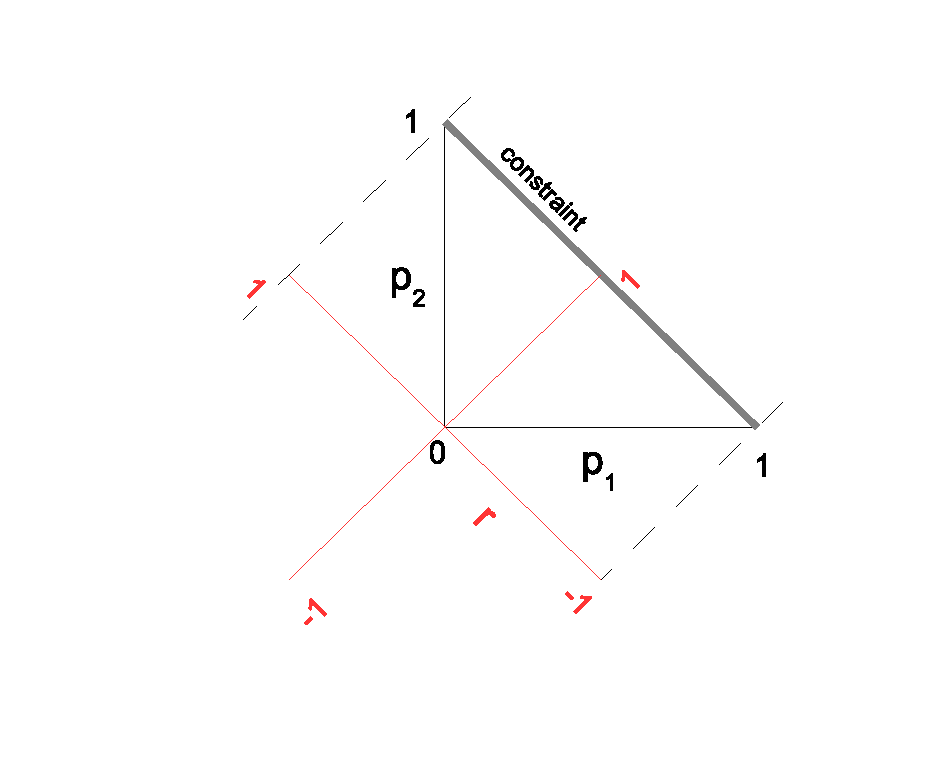
\includegraphics[width=0.6\textwidth]{../multi2/binary_class_map}
\end{center}

\section*{Abstract}

\input{orthogonal_abstract.txt}

\section*{Keywords}
\textbf{multi-class classification, 
	conditional probabilities,
	SVM,
	error-correcting codes,
	constrained linear least squares}

\tableofcontents

\section*{List of symbols}
\addcontentsline{toc}{section}{List of symbols}

\begin{tabular}{lll}
symbol & description & first used \\\hline
	$c$ & class & (\ref{min_dist}) \\
	$\vec x$ & test point & (\ref{min_dist})\\
	$A = \lbrace a_{ij} \rbrace$ & coding matrix & (\ref{min_dist})\\
	$\vec r = \lbrace r_i \rbrace$ & vector of binary decision functions & (\ref{rdef}) \\
	$P_i(c | \vec x)$ & conditional probability of $i$th binary classifier & (\ref{rdef})\\
	$p_j = p(j | \vec x)$ & multi-class conditional probability & (\ref{multiclass})\\
	$m$ & number of classes & (\ref{multiclass})\\
	$n$ & number of binary classifiers & (\ref{multiclass}) \\
	$I$ & identity matrix & (\ref{orthogonal})\\
	$t$ & whole number for enumerating cases & Section \ref{construction} \\
	$p(\vec x)$ & prior distribution & (\ref{theorem}) \\
	$\lbrace \vec x_i:y_i \rbrace$ & a set of training samples & (\ref{theorem}) \\
	$N$ & number of training samples/conditional probabilities & (\ref{theorem})\\
	$\delta$ & Kronecker delta & (\ref{theorem}) \\
	$i_0$ & rank of first winning probability & (\ref{prob_val1})\\
\end{tabular}




\section{Introduction}

Many methods of statistical classication can only discriminate between two classes. 
Examples include lineear classifiers such as perceptrons and logistic regression \citep{Michie_etal1994}, 
piecewise linear classifiers \cite{Herman_Yeung1992},
as well as support vector machines \citep{kernel_intro}.
There are many ways of generalizing binary classification to 
multi-class.
Three of the most common are one versus one, one versus the rest and 
error-correcting coding matrices \citep{Hsu_Lin2002}.
Here we are interested in the error-correcting coding matrices
\citep{Dietterich_Bakiri1995, Windeatt_Ghaderi2002}.
Rather than use a random coding matrix here we are interested in one that is
more carefully designed.

In error-correcting coding, there is a coding matrix, $A$, that specifies
how the set of multiple classes is partitioned.
Typically, the class of the test point is determined by the distance between
a column in the matrix and a vector of binary decision functions:
\begin{equation}
	c(\vec x) = \arg \min_j | \vec a^{(j)} - \vec r(\vec x) |
\end{equation}
where $\vec a^{(j)}$ is the $j$th column of the coding matrix.
If we take the upright brackets as a Euclidean distance, and assume that
each partition partitions all of the classes, that is, there are no zeroes
in $A$, then this reduces to a {\it voting} solution:
\begin{equation}
	c = \arg \max A^T \vec r \label{voting}
\end{equation}
Both \citet{Allwein_etal2000} and \citet{Windeatt_Ghaderi2002} show that to
maximize the accuracy of an error-correcting coding matrix, the distance
between each column, $|\vec a^{(i)} - \vec a^{(j)}|_{i \ne j}$ should be as
large as possible.
Using the same assumptions, this reduces to:
\begin{equation}
	\min |\vec a^{(i)} \cdot a^{(j)}|_{i \ne j}
\end{equation}
In other words, the coding matrix, $A$, should be orthogonal.
This approach to the multi-class problem will be described in detail in this note.

\section{Algorithm}

We wish to design a set of $m$ binary classifiers, each of which return a 
decision function:
\begin{equation}
r_j(\vec x) = P_i(-1 | \vec x) - P_i(+1 | \vec x)
\end{equation}
where $P_i(c | \vec x)$ is the conditional probability of the $c$th class of
the $i$th classifier.
Each binary classifier partitions a set of i$n$ classes such that for a
given test point, $\vec x$:
\begin{equation}
\sum_j a_{ij} p_j = r_j
\end{equation}
where $A=\lbrace a_{ij} \in \lbrace -1, +1 \rbrace  \rbrace$ is a {\it coding
matrix} and $p_j = p(j | \vec x)$ is the conditional probability of the $j$th
class.
In vector notation:
\begin{equation}
	A \vec p = \vec r \label{inverse}
\end{equation}
The more general case where a class can be excluded, that is each element of 
the coding matrix is, $a_{ij} \in \lbrace -1, 0, +1\rbrace$, 
will not be addressed here.

Note that this assumes that the binary decision functions, $\vec r$,
estimate the conditional probabilities perfectly.
In practice
there are a set of constrainsts that must be enforced
because $\vec p$ is only allowed to take on certain values.
Thus, we wish to solve the following minimization problem:
\begin{eqnarray}
	\vec p & = & \arg \min_{\vec p} | A \vec p - \vec r | \label{minimization}\\
	\sum_j p_j & = & 1 \label{normalization}\\
	p_j & \ge & 0 \label{nonnegative}
\end{eqnarray}

The unconstrained minimization problem is trivially easy to solve
if $A$ is orthogonal:
\begin{equation}
	A^T A = n I
\end{equation}
where $I$ is the $n \times n$ identity matrix.
Note that the voting solution in (\ref{voting}) is now equivalent to
the inverse solution in (\ref{inverse}).
This allows us to determine the class easily, but we also wish to solve for
the probabilities, $\vec p$, so that none of the constraints in 
(\ref{normalization}) or (\ref{nonnegative}) are violated.

The orthogonality property allows us to reduce the minimization problem 
in (\ref{minimization}) to something much simpler:
\begin{equation}
	\vec p = \arg \min_{\vec p} | \vec p - \vec p_0 |
\end{equation}
where $p_0 = A^T \vec r/n$ with the constraints in (\ref{normalization}) and
(\ref{nonnegative}) remaining the same.
Because the system has been rotated and expanded, the non-negativity 
constraints in (\ref{nonnegative}) remain orthogonal, meaning they are 
independent: enforcing one by setting one of the probabilities to zero, 
$p_k=0$ for example, shouldn't otherwise affect the solution.
This still leaves the normalization constraint in (\ref{normalization}):
the problem, now strictly geometrical, is comprised of finding the point nearest $p_0$ on the diagonal hyper-surface that bisects the unit hyper-cube.

Briefly, we can summarize the algorithm as follows:
1. move to the nearest point that satisfies the normalization constraint,
(\ref{normalization}); 2. if one or more of the probabilities is negative,
move to the nearest point that satisfies both these and the normalization
constraint; 3. repeat step 2.
More specifically, let $\vec 1$ be a vector of all $1$'s:
\begin{itemize}
	\item $n_0=n$
	\item while $\exists k \, p_{ik} \le 0 \lor \vec p_i \cdot \vec 1 \ne 1$:
	\begin{itemize}
		\item if $\vec p_i \cdot \vec 1 \ne 1$ then 
		$\vec p_{i+1} = \vec p_i + (\vec p_i \cdot \vec 1 - 1)/n_i$
		\item let $K$ be the set of $k$ such that $p_{i+1,k} < 0$
		\item for each $k$ in $K$:
		\begin{itemize}
			\item $p_{i+1,k}=0$
			\item Remove $k$ from the problem
		\end{itemize}
		\item $n_{i+1}=n_i-|K|$
		\item $i=i+1$
	\end{itemize}
\end{itemize}

Note that the direction vectors form an orthogonal set.
For instance, suppose $n_0=4$ and after enforcing the normalization constraint,
the first probability is less than zero, $p_{1,1} < 0$,
then the direction vectors for the two motions are:
\begin{equation}
	\frac{1}{2}[1, 1, 1, 1] \cdot \frac{1}{2\sqrt{3}} [-3, 1, 1, 1] = 0
\end{equation}

More formally, consider the following sequence of vectors:
\begin{equation}
	v_{ij} = \frac{1}{\sqrt{(n-i)^2-n+i}} \left \lbrace \begin{array}{rl}
			0; & j < i \\
			-n+i+1; & j=i \\
			1; & j > i
		\end{array} \right .
\end{equation}
where $j \in [1, n]$.


\section{Constructing the coding matrix}

An obvious method of designing an orthogonal $A$ is using harmonic series.
Consider the following matrix for eight binary classifiers ($m=8$) and
five classes ($n=5$):
\begin{equation}
	A^T = \left [ \begin{array}{rrrrrrrr}
			-1 & -1 & -1 & -1 & 1 & 1 & 1 & 1 \\
			-1 & -1 & 1 & 1 & 1 & 1 & -1 & -1 \\
			-1 & -1 & 1 & 1 & -1 & -1 & 1 & 1 \\
			-1 & 1 & 1 & -1 & -1 & 1 & 1 & -1 \\
			-1 & 1 & -1 & 1 & -1 & 1 & -1 & 1
	\end{array} \right ]
\end{equation}
This will limit the size of $m$ relative to $n$; more precisely:
$m=2 \log_2 n - 1$.

Finding an $A$ such that $A^T A = n I$ and $a_{ij} \in \lbrace -1, 1, \rbrace$
is quite a difficult combinatorial problem.
Noting which versions of $A$ are degenerate (equivalent) can help us whittle
away at the problem:
\begin{itemize}
	\item $-A$ is equivalent to $A$
	\item re-arranging either the rows or columns of $A$ makes an equivalent $A$: $T_{ij} A$ or $A T_{ij}^T$ are both equivalent to $A$ where $T_{ij}$ is the elementary matrix which exchanges rows $i$ and $j$
\end{itemize}

The most efficient method I've discovered so far of constructing an orthogonal
coding matrix is based on a generalization of the cross-product:
each time a new vector is added to the set of mutually orthogonal vectors, 
the sub-space of possible new members is decreased by one.
Thus, if there are $k$ vectors of length $m$ already, then we need only specify $m-k$
of the elements of any new vector.
We can solve for the rest of the elements using sub-matrices:
\begin{equation}
	\sum_{i=1}^{k} a_{ij} v_i = - \sum_{i=k+1}^m a_{ij} v_i
\end{equation}
where $\vec v$ is the candidate new vector of which we have specified the last
$m-k$ elements: there will of course be $2^{m-k}$ possibilities.
If $v_i \in \lbrace -1, +1 \rbrace;~i=[1..k]$ then we have found a new 
column of the matrix.

With this algorithm, you will have to examine $2^{m(m+1)/2}$ combinations
maximum.
With a pure, brute force algorithm, this would be $2^{m^2-1}$ to examine all
permutations while for a similarly brute force but combinatorial algorithm 
in which all possible vectors are treated as elements to be chosen for the 
final matrix this would be $2^{m-1}$ choose $m$ or:
\begin{equation}
	\frac{2^{m-1}!}{m!(2^{m-1}-m)!}
\end{equation}
By taking advantage of the negative degeneracy (first point, above) 
we reduce both these algorithms by half, hence the use of $m-1$ instead of $m$.

The final point concerns the size of $m$. In order to find on the order
of $n=m$ columns to match the $m$ rows, it appears that $m$ should be 
(at minimum) divisible by $4$: $m \mathrm{mod} 4 = 0$.
Note that we can have more rows than columns but not the other way around.

\section{Validating the probabilities}

Since the main goal of the method 
is to solve for the conditional probabilities, 
we need a good way to validate them. 
Here we use a technique based on the
following theorem, which can be derived from Bayes theorem and the 
definition of probability:
\begin{equation}
	\lim_{n \rightarrow \infty} \sum_{i=0}^n \left [
	p(c | \vec x) - \delta_{cy_i} \right ] = 0
	\label{theorem}
\end{equation}
where $\delta$ is the Kronecker delta.
To make this useful for real problems we need to do several things.
First, the probability estimates are sorted with regard to the class
label, as follows:
\begin{equation}
	p(c_{i+1} | \vec x_{i+1}) \ge p(c_i | \vec x_i)
\end{equation}
Second, we rearrange Equation (\ref{theorem}) as follows:
\begin{equation}
	n - i_0 \approx \sum_{i|p \ge 1/m}^{n} \frac{\delta_{c_i y_i}}{p(c_i | \vec x_i)}
\end{equation}
In other words, if the probabilities are well estimated, the RHS should
follow, on average, single step intervals at each step in the trace.
Finally, to prevent singularities at the bottom end, 
we divide it into two parts:
one for all the probabilities greater than $1/m$, above, and one for all those 
less than $1/m$, below:
\begin{equation}
	n - i_0  \approx \sum_{i=n}^{p < 1/m} \frac{\delta_{c_i y_i} - 1}{1 - p(c_i | \vec x_i)}
\end{equation}
where $i_0$ is defined such that:
\begin{equation}
	\left \lbrace
	\begin{matrix}
		p(c_i | \vec x_i) & \ge & 1/m &| i \ge i_0 \\
		p(c_i | \vec x_i) & < & 1/m & | i < i_0
	\end{matrix}
	\right .
\end{equation}
We use the correlation coefficient to gauge the accuracy and the slope to
measure the bias.
This method of validating conditional probabilities was used in
\citet{Mills2009} for a binary classification problem.




\appendix

\section*{Acknowledgements}

Thanks to Chih-Chung Chan and Chih-Jen Lin of the National Taiwan University
for data from the LIBSVM archive and also to David Aha and the curators of
the UCI Machine Learning Repository for statistical classification datasets.

\newpage
\addcontentsline{toc}{section}{References}
\bibliography{../agf_bib,../pwl,../datasets,orthogonal}

\end{document}
